% !TeX root = main.tex

\chapter{随机事件及其概率}
\thispagestyle{plain}

\section{随机事件}

\question 写出下列随机试验的样本空间:

(1)抛一枚硬币,观察正面和反面出现的情况;

(2)抛三枚硬币,观察正面和反面出现的情况;

(3)连续抛一枚硬币,直至出现正面为止;

(4)抛一枚骰子,观察出现的点数;

(5)抛两枚骰子,观察出现的点数;

(6)抛两枚骰子,记录出现的点数之和;

(7)在一个箱子中装有10个同型号的某种零件,其中有3个次品和7个合格品,从该箱子中任取3个零件,观察其中次品的个数;

(8)记录某机场在一天内收到咨询电话的次数;

(9)测试电视机的寿命;

(10)口袋中有黑、白、红球各一个,从中任取两个球;先从中取出一个,放回后再取出一个;

(11)口袋中有黑、白、红球各一个,从中任取两个球;先从中取出一个,不放回后再取出一个.

\begin{solution}
    (1) $\varOmega = \{ 0, 1 \}$,其中 $0$ 表示反面, $1$ 表示正面.

    (2) $\varOmega = \{ (0,0,0), (0,0,1), (0,1,0), (0,1,1), (1,0,0), (1,0,1), (1,1,0), (1,1,1) \}$

    (3) $\varOmega = \{ (1), (0,1), (0,0,1), (0,0,0,1), \cdots \}$

    (4) $\varOmega = \{ 1,2,3,4,5,6 \}$

    (5) $\varOmega = \{ (x,y) \mid x,y = 1,2,3,4,5,6 \}$

    (6) $\varOmega = \{ 2, 3, 4, \cdots, 12 \}$

    (7) $\varOmega = \{ 0,1,2,3 \}$

    (8) $\varOmega = \{ 0,1,2,3,\cdots \}$

    (9) $\varOmega = [0, +\infty)$

    (10) $\varOmega = \{ \text{黑黑}, \text{黑白}, \text{黑红}, \text{白黑}, \text{白白}, \text{白红}, \text{红黑}, \text{红白}, \text{红红} \}$

    (11) $\varOmega = \{ \text{黑白}, \text{黑红}, \text{白黑}, \text{白红}, \text{红黑}, \text{红白} \}$
\end{solution}

\question 设 $A,B,C$ 为三事件,试表示下列事件:

(1) $A$ 发生, $B,C$ 不发生;

(2) $A,B,C$ 都发生;

(3) $A,B,C$ 都不发生;

(4) $A,B,C$ 中只有一个发生;

(5) $A,B,C$ 中至少有一个发生;

(6) $A,B,C$ 中至多有一个发生;

(7) $A,B,C$ 中至少有一个不发生;

(8) $A,B,C$ 中至多有两个发生;

(9) $A,B,C$ 中至少有两个发生;

(10) $A,B,C$ 中恰好有两个发生.

\begin{solution}
    (1) $A \, \overline{B} \, \overline{C}$

    (2) $ABC$

    (3) $\overline{A} \, \overline{B} \, \overline{C}$

    (4) $A \, \overline{B} \, \overline{C} \cup \overline{A} B \overline{C} \cup \overline{A} \, \overline{B} \, C$

    (5) $\varOmega - \overline{A} \, \overline{B} \, \overline{C} = \overline{\overline{A} \, \overline{B} \, \overline{C}} = A \cup B \cup C$

    (6) $\overline{A} \, \overline{B} \, \overline{C} \cup A \, \overline{B} \, \overline{C} \cup \overline{A} B \overline{C} \cup \overline{A} \, \overline{B} \, C$

    (7) $\overline{A} \cup \overline{B} \cup \overline{C}$

    (8) $\varOmega - ABC = \overline{ABC} = \overline{A} \cup \overline{B} \cup \overline{C}$

    (9) $AB \cup AC \cup BC$

    (10) $AB \overline{C} \cup A \overline{B} C \cup \overline{A} BC$
\end{solution}

\question 判断下列命题是否成立:

(1) $A-(B-C) = (A-B) \cup C$;

(2)若 $AB = \text{\O}$ 且 $C \subseteq A$,则 $BC = \text{\O}$;

(3) $(A \cup B) - B = A$;

(4) $(A - B) \cup B = A$.

\begin{solution}
    (1)
    $$
    \begin{aligned}
        A-(B-C) &= A - B \overline{C} \\
        &= A \overline{B \overline{C}} \\
        &= A (\overline{B} \cup C) \\
        &= (A \overline{B}) \cup (AC) \\
        &= (A-B) \cup (AC) \\
        & \not= (A-B) \cup C
    \end{aligned}
    $$
    命题1不成立.

    (2)成立.

    (3)
    $$
    (A \cup B) - B = (A \cup B) \overline{B} = (A \overline{B}) \cup (B \overline{B}) = A \overline{B} \not= A
    $$
    命题3不成立.

    (4)
    $$
    (A - B) \cup B = (A \overline{B}) \cup B = (A \cup B)(\overline{B} \cup B) = A \cup B \not= A
    $$
    命题4不成立.
\end{solution}

\vspace{1em}

\question 证明下列事件的运算公式:

(1) $A = AB \cup A \overline{B}$;

(2) $A \cup B = A \cup \overline{A} B$.

\begin{proof}
    (1) $AB \cup A \overline{B} = A(B \cup \overline{B}) = A \varOmega = A$

    (2) 由(1)可得 $B = AB \cup \overline{A} B$,因此
    $$
    \begin{aligned}
        A \cup B &= A \cup (AB \cup \overline{A} B) \\
        &= (A \cup AB) \cup \overline{A} B \\
        &= A(\varOmega \cup B) \cup \overline{A} B \\
        &= A \cup \overline{A} B
    \end{aligned}
    $$
\end{proof}

\section{随机事件的概率}

%===================== 概率的定义和性质 =====================

\question 设 $A,B$ 是同一个试验中的两个事件, $P(A)=0.6, P(A-B)=0.2, P(A \cup B) = 0.9$.求 $P(\overline{AB}), P(B), P((\overline{A} \cup B)(A \cup \overline{B}))$.

\begin{solution}
    由于 $P(A-B) = P(A) - P(AB)$,所以
    $$
    P(AB) = P(A) - P(A-B) = 0.6 - 0.2 = 0.4
    $$
    进而可得
    $$
    P(\overline{AB}) = 1 - P(AB) = 1 - 0.4 = 0.6
    $$

    由于 $P(A \cup B) = P(A) + P(B) - P(AB)$,所以
    $$
    P(B) = P(A \cup B) - P(A) + P(AB) = 0.9 - 0.6 + 0.4 = 0.7
    $$

    由随机事件的运算性质可得
    $$
    \begin{aligned}
        (\overline{A} \cup B)(A \cup \overline{B}) &= [(\overline{A} \cup B) A] \cup [(\overline{A} \cup B) \overline{B}] \\
        &= (A \overline{A}) \cup (AB) \cup (\overline{A} \, \overline{B}) \cup (B \overline{B}) \\
        &= (AB) \cup (\overline{A \cup B})
    \end{aligned}
    $$
    又因为 $(AB)(\overline{A \cup B}) = (AB)(\overline{A} \, \overline{B}) = \text{\O}$,所以
    $$
    \begin{aligned}
        P((\overline{A} \cup B)(A \cup \overline{B})) &= P((AB) \cup (\overline{A \cup B})) \\
        &= P(AB) + P(\overline{A \cup B}) \\
        &= P(AB) + 1 - P(A \cup B) \\
        &= 0.4 + 1 - 0.9 \\
        &= 0.5
    \end{aligned}
    $$
\end{solution}

\vspace{1em}

\question 设 $A$ 和 $B$ 是同一试验 $E$ 的两个随机事件,证明: $1 - P(\overline{A}) - P(\overline{B}) \leqslant P(AB) \leqslant P(A \cup B)$.

\begin{proof}
    因为 $AB \subseteq A \subseteq (A \cup B)$,所以
    $$
    P(AB) \leqslant P(A \cup B)
    $$

    因为
    $$
    1 - P(AB) = P(\overline{AB}) = P(\overline{A} \cup \overline{B}) \leqslant P(\overline{A}) + P(\overline{B})
    $$
    所以
    $$
    1 - P(\overline{A}) - P(\overline{B}) \leqslant P(AB)
    $$
\end{proof}

\question 已知 $P(A) = P(B) = P(C) = \dfrac{1}{4}, P(AB) = 0, P(AC) = P(BC) = \dfrac{1}{16}$.则 $A,B,C$ 中至少发生一个的概率是多少? $A,B,C$ 都不发生的概率是多少?

\begin{solution}
    因为 $P(AB) = 0$,且 $ABC \subseteq AB$,由概率的单调性可知 $P(ABC) = 0$.由概率的加法公式可得 $A,B,C$ 中至少发生一个的概率为
    $$
    \begin{aligned}
        P(A \cup B \cup C) &= P(A) + P(B) + P(C) - P(AB) - P(BC) - P(AC) + P(ABC) \\
        &= \dfrac{1}{4} + \dfrac{1}{4} + \dfrac{1}{4} - 0 - \dfrac{1}{16} - \dfrac{1}{16} + 0 \\
        &= \dfrac{5}{8}
    \end{aligned}
    $$
    $A,B,C$ 都不发生的概率为
    $$
    \begin{aligned}
        P(\overline{A} \, \overline{B} \, \overline{C}) &= P(\overline{A \cup B \cup C}) \\
        &= 1 - P(A \cup B \cup C) \\
        &= 1 - \dfrac{5}{8} \\
        &= \dfrac{3}{8}
    \end{aligned}
    $$
\end{solution}

\question 设事件 $A$ 和 $B$ 互不相容,且 $P(A)=0.3, P(B)=0.5$,求以下事件的概率:

(1) $A$ 与 $B$ 中至少有一个发生;

(2) $A$ 和 $B$ 都发生;

(3) $A$ 发生但 $B$ 不发生.

\begin{solution}
    因为 $A$ 和 $B$ 互不相容,所以 $AB = \text{\O}, P(AB)=0$.

    (1) $P(A \cup B) = P(A) + P(B) = 0.3+0.5 = 0.8$

    (2) $P(AB) = 0$

    (3) $P(A-B) = P(A) - P(AB) = P(A) = 0.3$
\end{solution}

\question 某城市中共发行3种报纸A, B, C.在这城市的居民中有45\%订阅A报、35\%订阅B报、30\%订阅C报, 10\%同时订阅A报B报、8\%同时订阅A报C报、5\%同时订阅B报C报、3\%同时订阅A, B, C报.求以下事件的概率:

(1)只订阅A报的;

(2)只订阅一种报纸的;

(3)至少订阅一种报纸的;

(4)不订阅任何一种报纸的.

\begin{solution}
    设事件 $A,B,C$ 分别表示订阅A, B, C报,根据条件可得 $P(A)=0.45, P(B)=0.35, P(C)=0.3, P(AB)=0.1, P(AC)=0.08, P(BC)=0.05, P(ABC)=0.03$.

    (1)
    $$
    \begin{aligned}
        P(\text{只订阅A报}) &= P(A \, \overline{B} \, \overline{C}) \\
        &= P(A (\overline{B \cup C})) \\
        &= P(A - (B \cup C)) \\
        &= P(A) - P(A(B \cup C)) \\
        &= P(A) - P(AB \cup AC) \\
        &= P(A) - [P(AB) + P(AC) - P(ABC)] \\
        &= 0.45 - (0.1+0.08-0.03) \\
        &= 0.3
    \end{aligned}
    $$

    (2)
    $$
    P(\text{只订阅一种报纸}) = P(A \, \overline{B} \, \overline{C}) + P(\overline{A} B \overline{C}) + P(\overline{A} \, \overline{B} \, C)
    $$
    其中
    $$
    \begin{aligned}
        & P(\overline{A} \, B \, \overline{C}) = P(B) - P(AB) - P(BC) + P(ABC) = 0.35-0.1-0.05+0.03 = 0.23 \\
        & P(\overline{A} \, \overline{B} \, C) = P(C) - P(AC) - P(BC) + P(ABC) = 0.3-0.08-0.05+0.03 = 0.2
    \end{aligned}
    $$
    因此
    $$
    P(\text{只订阅一种报纸}) = 0.3 + 0.23 + 0.2 = 0.73
    $$

    (3)
    $$
    \begin{aligned}
        P(\text{至少订阅一种报纸}) &= P(A \cup B \cup C) \\
        &= P(A) + P(B) + P(C) - P(AB) - P(BC) - P(AC) + P(ABC) \\
        &= 0.45 + 0.35 + 0.3 - 0.1 - 0.05 - 0.08 + 0.03 \\
        &=0.9
    \end{aligned}
    $$

    (4) $P(\text{不订阅任何一种报纸}) = P(\overline{A \cup B \cup C}) = 1 - P(A \cup B \cup C) = 1-0.9 = 0.1$
\end{solution}

%===================== 古典概型 =====================

\question 抛两枚硬币,求出现一个正面一个反面的概率.

\begin{solution}
    此试验的样本空间为 $\varOmega = \{ (\text{正}, \text{正}), (\text{正}, \text{反}), (\text{反}, \text{正}), (\text{反}, \text{反}) \}$,样本点的个数为4,且每个样本点发生的可能性是相等的.事件``出现一个正面一个反面"含有的样本点个数为2,根据古典概型可得该事件发生的概率为 $\dfrac{1}{2}$.
\end{solution}

\begin{note}
    \indent 如果将样本空间写成 $\varOmega' = \{ (\text{正}, \text{正}), (\text{反}, \text{反}), (\text{一正一反}) \}$,这3个样本点不是等可能的,不满足古典概型的条件.
\end{note}

\question 任取两个正整数,求它们的和为偶数的概率.

\begin{solution}
    记取出偶数为``0",取出奇数为``1",则随机试验``任取两个正整数"的样本空间为
    $$
    \varOmega = \{ (0,0), (0,1), (1,0), (1,1) \}
    $$
    令事件 $A$ 表示``取出的两个正整数之和为偶数",则 $A = \{ (0,0), (1,1) \}$,从而所求概率为 $$P(A) = \dfrac{1}{2}$$
\end{solution}

\question 从 $n$ 个数字 $1,2,\cdots,n$ 中任取3个,求大小在中间的数字恰好为 $k \, (1 < k < n)$ 的概率.

\begin{solution}
    从 $n$ 个数字中任取3个,共有 $\mathrm{C}_{n}^3$ 种取法.如果大小在中间的数字恰好为 $k$,必须有一个小于 $k$、一个等于 $k$、一个大于 $k$,这样的取法有 $\mathrm{C}_{k-1}^1 \mathrm{C}_1^1 \mathrm{C}_{n-k}^1$ 种.因此所求概率为
    $$
    p = \dfrac{\mathrm{C}_{k-1}^1 \mathrm{C}_1^1 \mathrm{C}_{n-k}^1}{\mathrm{C}_{n}^3} = \dfrac{6(k-1)(n-k)}{n(n-1)(n-2)}
    $$
\end{solution}

\question 从 $0, 1, 2, \cdots, 9$ 十个数字中任意选出三个不同的数字,求下列事件的概率:

(1) $A_1=$ ``三个数字中不含0和5'';

(2) $A_2=$ ``三个数字中不含0或5'';

(3) $A_3=$ ``三个数字中含0但不含5''.

\begin{solution}
    从十个数字中任意选出三个不同的数字,共有 $\mathrm{C}_{10}^3$ 种取法.

    (1)要使事件 $A_1$ 发生,可以从0和5之外的八个数字中选出三个数字,有 $\mathrm{C}_8^3$ 种取法.因此
    $$
    P(A_1) = \dfrac{\mathrm{C}_8^3}{\mathrm{C}_{10}^3} = \dfrac{7}{15}
    $$

    (2)设事件 $A=$ ``三个数字中不含0'', $B=$ ``三个数字中不含5'',则
    $$
    \begin{aligned}
        & P(A) = P(B) = \dfrac{\mathrm{C}_9^3}{\mathrm{C}_{10}^3} = \dfrac{7}{10} \\
        & P(AB) = P(A_1) = \dfrac{7}{15}
    \end{aligned}
    $$
    进而有
    $$
    P(A_2) = P(A \cup B) = P(A) + P(B) - P(AB) = \dfrac{7}{10} + \dfrac{7}{10} - \dfrac{7}{15} = \dfrac{14}{15}
    $$

    (3)要使事件 $A_3$ 发生,可以先选出0,再从0和5之外的八个数字中选出两个数字,有 $\mathrm{C}_8^2$ 种取法.因此
    $$
    P(A_3) = \dfrac{\mathrm{C}_8^2}{\mathrm{C}_{10}^3} = \dfrac{7}{30}
    $$
\end{solution}

\question 将15名新生(其中有3名优秀生)随机地分配到3个班级去,其中一班4名,二班5名,三班6名.求:

(1)每个班级各分配到一名优秀生的概率;

(2) 3名优秀生分配到一个指定班级的概率;

(3) 3名优秀生分配到同一个班级的概率.

\begin{solution}
    将15名新生随机地分配给一班4名、二班5名、三班6名,共有 $\mathrm{C}_{15}^4 \mathrm{C}_{11}^5 \mathrm{C}_6^6$ 种分法.

    (1)将3名优秀生分配到三个班级的分法共有 $\mathrm{A}_3^3$ 种,将其余12名新生分配给一班3名、二班4名、三班5名的分法共有 $\mathrm{C}_{12}^3 \mathrm{C}_9^4 \mathrm{C}_5^5$ 种,则每个班级各分配到一名优秀生的分法共有 $\mathrm{A}_3^3 \mathrm{C}_{12}^3 \mathrm{C}_9^4 \mathrm{C}_5^5$ 种.因此所求概率为
    $$
    p = \dfrac{\mathrm{A}_3^3 \mathrm{C}_{12}^3 \mathrm{C}_9^4 \mathrm{C}_5^5}{\mathrm{C}_{15}^4 \mathrm{C}_{11}^5 \mathrm{C}_6^6} = \dfrac{24}{91}
    $$

    (2)如果将3名优秀生分配到一班,则其余12名新生将分配给一班1名、二班5名、三班6名,此时分法共有 $\mathrm{C}_{12}^1 \mathrm{C}_{11}^5 \mathrm{C}_6^6$ 种,所求概率为
    $$
    p_1 = \dfrac{\mathrm{C}_{12}^1 \mathrm{C}_{11}^5 \mathrm{C}_6^6}{\mathrm{C}_{15}^4 \mathrm{C}_{11}^5 \mathrm{C}_6^6} = \dfrac{4}{455}
    $$

    如果将3名优秀生分配到二班,则其余12名新生将分配给一班4名、二班2名、三班6名,此时分法共有 $\mathrm{C}_{12}^4 \mathrm{C}_{8}^2 \mathrm{C}_6^6$ 种,所求概率为
    $$
    p_2 = \dfrac{\mathrm{C}_{12}^4 \mathrm{C}_{8}^2 \mathrm{C}_6^6}{\mathrm{C}_{15}^4 \mathrm{C}_{11}^5 \mathrm{C}_6^6} = \dfrac{2}{91}
    $$

    如果将3名优秀生分配到三班,则其余12名新生将分配给一班4名、二班5名、三班3名,此时分法共有 $\mathrm{C}_{12}^4 \mathrm{C}_{8}^5 \mathrm{C}_3^3$ 种,所求概率为
    $$
    p_3 = \dfrac{\mathrm{C}_{12}^4 \mathrm{C}_{8}^5 \mathrm{C}_3^3}{\mathrm{C}_{15}^4 \mathrm{C}_{11}^5 \mathrm{C}_6^6} = \dfrac{4}{91}
    $$

    (3)用 $A_i$ 表示``3名优秀生全部分配到 $i$ 班" $(i=1,2,3)$,则事件``3名优秀生分配到同一个班级"可以表示为 $A_1 \cup A_2 \cup A_3$.又因为 $A_i A_j = \text{\O} \, (i \not= j, i,j=1,2,3)$,所以所求概率为
    $$
    p = P(A_1 \cup A_2 \cup A_3) = P(A_1) + P(A_2) + P(A_3) = \dfrac{4}{455} + \dfrac{2}{91} + \dfrac{4}{91} = \dfrac{34}{455}
    $$
\end{solution}

\question 抛两颗骰子,求下列事件的概率:

(1)点数之和为6;

(2)点数之和不超过6;

(3)至少有一个6点.

\begin{solution}
    抛两颗骰子所得点数的样本空间为 $\varOmega = \{ (x,y) \mid x,y=1,2,3,4,5,6 \}$,样本点数量为36.

    (1)令事件 $A$ 为``点数之和为6",则
    $$
    A = \{ (1,5), (2,4), (3,3), (4,2), (5,1) \}
    $$
    所以所求概率为
    $$
    P(A) = \dfrac{5}{36}
    $$

    (2)令事件 $B$ 为``点数之和不超过6",则
    $$
    \begin{aligned}
        B = \{ & (1,1), (1,2), (1,3), (1,4), (1,5), (2,1), (2,2), (2,3), \\
        & (2,4), (3,1), (3,2), (3,3), (4,1), (4,2), (5,1) \}
    \end{aligned}
    $$
    所以所求概率为
    $$
    P(B) = \dfrac{15}{36} = \dfrac{5}{12}
    $$

    (3)令事件 $C$ 为``至少有一个6点",则
    $$
    \begin{aligned}
        C = \{ & (1,6), (2,6), (3,6), (4,6), (5,6), (6,6), \\
        & (6,1), (6,2), (6,3), (6,4), (6,5) \}
    \end{aligned}
    $$
    所以所求概率为
    $$
    P(C) = \dfrac{11}{36}
    $$
\end{solution}

\question 考虑一元二次方程 $x^2 + Bx + C = 0$,其中 $B,C$ 分别是将一颗骰子连续抛两次先后出现的点数,求该方程有实根的概率 $p$ 和有重根的概率 $q$.

\begin{solution}
    将一颗骰子连续抛两次所得点数的样本空间为 $\varOmega = \{ (B,C) \mid B,C=1,2,3,4,5,6 \}$,样本点数量为36.
    
    事件``该方程有实根"发生的条件为 $B^2 - 4C \geqslant 0$,而
    $$
    \begin{aligned}
        \{ B^2 - 4C \geqslant 0 \} = \{ & (2,1), (3,1), (4,1), (5,1), (6,1), (3,2), (4,2), (5,2), (6,2), \\
        & (4,3), (5,3), (6,3), (4,4), (5,4), (6,4), (5,5), (6,5), (5,6), (6,6) \}
    \end{aligned}
    $$
    共有19个样本点,因此
    $$
    p = P(B^2 - 4C \geqslant 0) = \dfrac{19}{36}
    $$

    事件``该方程有重根"发生的条件为 $B^2 - 4C = 0$,而
    $$
    \begin{aligned}
        \{ B^2 - 4C = 0 \} = \{ & (2,1), (4,4) \}
    \end{aligned}
    $$
    共有2个样本点,因此
    $$
    q = P(B^2 - 4C = 0) = \dfrac{2}{36} = \dfrac{1}{18}
    $$
\end{solution}

\question 从 $N$ 个数字 $1,2,\cdots,N$ 中可重复地随机抽取 $n$ 次,求抽到的最大数字正好为 $k \, (1 \leqslant k \leqslant N)$ 的概率.

\begin{solution}
    从 $N$ 个数字中可重复地抽取 $n$ 次,共有 $N^n$ 种取法.

    记事件 $B_i$ 为``抽到的最大数字小于等于 $i$'' ($i=1,2,\cdots,N$),则 $B_i$ 发生只需每次从 $1,2,\cdots,i$ 中取数即可,共有 $i^n$ 种取法,由古典概型可知
    $$
    P(B_i) = \dfrac{i^n}{N^n}
    $$

    记事件 $A_k$ 为``抽到的最大数字正好为 $k$",则 $A_k = B_k - B_{k-1}$,且 $B_{k-1} \subseteq B_k$,因此
    $$
    \begin{aligned}
        P(A_k) &= P(B_k - B_{k-1}) \\
        &= P(B_k) - P(B_{k-1}) \\
        &= \dfrac{k^n}{N^n} - \dfrac{(k-1)^n}{N^n} \\
        &= \dfrac{k^n - (k-1)^n}{N^n}
    \end{aligned}
    $$
\end{solution}

\question 从一副52张的扑克牌中任取4张,求下列事件的概率:

(1)全是黑桃;

(2)同花;

(3)没有两张同一花色;

(4)同色.

\begin{solution}
    从52张扑克牌中任取4张的取法有 $\mathrm{C}_{52}^4$ 种.

    (1)一副扑克牌中有13张黑桃,从中取出4张的取法有 $\mathrm{C}_{13}^4$ 种,因此所求概率为
    $$
    p_1 = \dfrac{\mathrm{C}_{13}^4}{\mathrm{C}_{52}^4} = \dfrac{11}{4165}
    $$

    (2)取出的4张牌全是某一特定花色的取法有 $\mathrm{C}_{13}^4$ 种,而一副扑克牌有4种花色,则4张牌同花的取法有 $4 \mathrm{C}_{13}^4$ 种,因此所求概率为
    $$
    p_2 = \dfrac{4 \mathrm{C}_{13}^4}{\mathrm{C}_{52}^4} = \dfrac{44}{4165}
    $$

    (3)``没有两张同一花色"需要从4种花色中各取一张,取法有 $13^4$ 种,因此所求概率为
    $$
    p_3 = \dfrac{13^4}{\mathrm{C}_{52}^4} = \dfrac{2197}{20825}
    $$

    (4)一副扑克牌中有红色和黑色牌各26张,取出4张同色牌的取法有 $2 \mathrm{C}_{26}^4$ 种,因此所求概率为
    $$
    p_4 = \dfrac{2 \mathrm{C}_{26}^4}{\mathrm{C}_{52}^4} = \dfrac{92}{833}
    $$
\end{solution}

\question 把10本书任意地放在书架上,求其中指定的4本书放在一起的概率.

\begin{solution}
    把10本书任意地放在书架上,共有 $\mathrm{A}_{10}^{10}$ 种放法.当其中指定的4本书放在一起时,将这4本书看作一个整体,与其他6本书一起放在书架上,有 $\mathrm{A}_7^7$ 种放法;放在一起的4本书又有不同的顺序,有 $\mathrm{A}_4^4$ 种放法.因此``其中指定的4本书放在一起''共有 $\mathrm{A}_7^7 \mathrm{A}_4^4$ 种放法,所求概率为
    $$
    p = \dfrac{\mathrm{A}_7^7 \mathrm{A}_4^4}{\mathrm{A}_{10}^{10}} = \dfrac{7! \times 4!}{10!} = \dfrac{1}{30}
    $$
\end{solution}

\question $n$ 个人随机地围一圆桌而坐,求甲、乙两人相邻而坐的概率.

\begin{solution}

    \textbf{解法一:} $n$ 个人围坐,共有 $\dfrac{\mathrm{A}_n^n}{n} = (n-1)!$ 种坐法.当甲、乙两人相邻而坐时,将甲、乙两人看作整体,有 $\dfrac{\mathrm{A}_{n-1}^{n-1}}{n-1} \mathrm{A}_2^2 = 2(n-2)!$ 种坐法.因此所求概率为
    $$
    p = \dfrac{2(n-2)!}{(n-1)!} = \dfrac{2}{n-1}
    $$

    \textbf{解法二:}设甲先坐好,再考虑乙的坐法.此时乙总共有 $n-1$ 个位置可坐,且这 $n-1$ 个位置都是等可能的,而乙与甲相邻有2个位置,因此所求概率为
    $$
    p = \dfrac{2}{n-1}
    $$
\end{solution}

\question 同时掷5枚骰子,求下列事件的概率:

(1)每枚都不一样;

(2)其中2枚相同(成对),另外3枚各不相同且与成对的2枚也不同;

(3)出现两组成对的骰子;

(4)其中3枚相同,另外2枚不同;

(5)其中4枚相同;

(6) 5枚全部相同.

\begin{solution}
    同时掷5枚骰子共有 $6^5$ 种不同情况.

    \vspace{0.3em}

    (1) $p_1 = \dfrac{6 \times 5 \times 4 \times 3 \times 2}{6^5} = \dfrac{5}{54}$

    \vspace{0.3em}

    (2) $p_2 = \dfrac{\mathrm{C}_5^2 \times 6 \times 5 \times 4 \times 3}{6^5} = \dfrac{25}{54}$

    \vspace{0.3em}

    (3)将5枚骰子分成3组,其中2组包含2枚骰子,另外一组只有1个骰子,这样的分法有 $\dfrac{\mathrm{C}_5^2 \mathrm{C}_3^2}{2} = 15$ 种.这三组骰子出现的点数不同,有 $6 \times 5 \times 4 = 120$ 种情况,因此所求概率为
    $$
    p_3 = \dfrac{15 \times 120}{6^5} = \dfrac{25}{108}
    $$

    (4) $p_4 = \dfrac{\mathrm{C}_5^3 \times 6 \times 5 \times 4}{6^5} = \dfrac{25}{162}$

    \vspace{0.3em}

    (5) $p_5 = \dfrac{\mathrm{C}_5^4 \times 6 \times 5}{6^5} = \dfrac{25}{1296}$

    (6) $p_6 = \dfrac{6}{6^5} = \dfrac{1}{1296}$
\end{solution}

\question[接草成环问题] 把 $2n$ 根草紧握在手中,仅露出它们的头和尾,然后随机地把 $2n$ 个头两两相接, $2n$ 个尾也两两相接.求放开手后 $2n$ 根草恰巧连成一个环的概率.

\begin{solution}
    先将头两两相接,此时所有接法都是等价的,如图 \ref{fig:例题-接草成环问题} 所示,所以只需考虑尾的接法.
    
    $2n$ 个尾两两相接,先任选1个尾,再从剩下的 $2n-1$ 个尾中任选1个尾相接;然后从剩下的 $2n-2$ 个尾中任选1个,与 $2n-3$ 个尾中的任意1个相接;以此类推,将 $2n$ 个尾两两相接共有 $2n (2n-1) (2n-2) (2n-3) \times \cdots \times 2 \times 1 = (2n)!$ 种方法.
    
    如果要成环,在从 $2n$ 个尾中任选1个之后,剩下的 $2n-1$ 个尾中有一个不能选择,所以只能从其余 $2n-2$ 个尾中任选1个相接;然后从剩下的 $2n-2$ 个尾中任选1个,与 $2n-4$ 个尾中的任意1个相接;以此类推,成环的方法共有 $2n (2n-2) (2n-2) (2n-4) \times \cdots \times 2 \times 1$ 种.因此所求概率为
    $$
    \begin{aligned}
        p &= \dfrac{2n (2n-2) (2n-2) (2n-4) \times \cdots \times 2 \times 1}{(2n)!} \\
        &= \dfrac{[2n (2n-2) (2n-4) \times \cdots \times 2] [(2n-2) (2n-4) \times \cdots \times 1]}{(2n)!} \\
        &= \dfrac{2^n n! \times 2^{n-1} (n-1)!}{(2n)!} \\
        &= \dfrac{2^{2n-1} n! (n-1)!}{(2n)!}
    \end{aligned}
    $$

    \begin{figure}[H]
        \centering

        \begin{tikzpicture}
            \def\xscale{1.5}
            % 端点
            \coordinate (A) at (0*\xscale, 0);
            \coordinate (A') at (0*\xscale, 2);
            \coordinate (B) at (1*\xscale, 0);
            \coordinate (B') at (1*\xscale, 2);
            \coordinate (C) at (2*\xscale, 0);
            \coordinate (C') at (2*\xscale, 2);
            \coordinate (D) at (3*\xscale, 0);
            \coordinate (D') at (3*\xscale, 2);
            \coordinate (E) at (5*\xscale, 0);
            \coordinate (E') at (5*\xscale, 2);
            \coordinate (F) at (6*\xscale, 0);
            \coordinate (F') at (6*\xscale, 2);
            \draw[fill] (A) circle (1.5pt);
            \draw[fill] (B) circle (1.5pt);
            \draw[fill] (C) circle (1.5pt);
            \draw[fill] (D) circle (1.5pt);
            \draw[fill] (E) circle (1.5pt);
            \draw[fill] (F) circle (1.5pt);
            \draw plot[mark=square*, mark size=1.5pt, only marks] coordinates {(A') (B') (C') (D') (E') (F')};

            % 草
            \draw (A) node[below]{1} -- (A') node[above]{$1'$};
            \draw (B) node[below]{2} -- (B') node[above]{$2'$};
            \draw (C) node[below]{3} -- (C') node[above]{$3'$};
            \draw (D) node[below]{4} -- (D') node[above]{$4'$};
            \draw (E) node[below]{$2n-1$} -- (E') node[above left]{$2n-1'$};
            \draw (F) node[below]{$2n$} -- (F') node[above right]{$2n'$};
            \node at (4*\xscale, 1) {$\cdots$};

            % 连接线
            \draw (A') .. controls (0.25*\xscale, 2.5) and (0.75*\xscale, 2.5) .. (B');
            \draw (C') .. controls (2.25*\xscale, 2.5) and (2.75*\xscale, 2.5) .. (D');
            \draw (E') .. controls (5.25*\xscale, 2.5) and (5.75*\xscale, 2.5) .. (F');
            \draw[dashed] (A) .. controls (0.5*\xscale, -0.5) .. (B);
            \draw (A) .. controls (0.5*\xscale, -1) and (1.5*\xscale, -1) .. (C);
            \node[cross out, draw, rotate=30] at (0.75*\xscale, -0.25) {};
        \end{tikzpicture}

        \caption{接草成环问题}
        \label{fig:例题-接草成环问题}
    \end{figure}
\end{solution}

\question\label{n个0与m个1} 把 $n$ 个``0''与 $m \, (m \leqslant n+1)$ 个``1''随机地排列,求没有两个``1''连在一起的概率.

\begin{solution}
    总共 $m+n$ 个位置,选择其中 $n$ 个放``0'',其余 $m$ 个位置放``1'',总的排列数为 $\mathrm{C}_{m+n}^n$.如果``没有两个`1'连在一起'',需要将``1''放在 $n$ 个``0''之间的空隙中,共有 $n+1$ 个位置,此时排列数为 $\mathrm{C}_{n+1}^m$.因此所求概率为
    $$
    p = \dfrac{\mathrm{C}_{n+1}^m}{\mathrm{C}_{m+n}^n} = \dfrac{n! (n+1)!}{(n-m+1)! (m+n)!}
    $$
\end{solution}

\question[插板法] 将 $n$ 个完全相同的球随机地放入 $N$ 个盒子中,求:

(1)某个指定的盒子中恰好有 $k \, (0 \leqslant k \leqslant n)$ 个球的概率;

(2)恰好有 $m \, (N-n \leqslant m \leqslant N-1)$ 个空盒的概率;

(3)某指定的 $m$ 个盒子中恰好有 $j$ 个球的概率.

\begin{solution}
    将 $n$ 个球排成一行,向其中插入 $N-1$ 块板,分成 $N$ 个区域,每个区域可以看成一个盒子.因此``将 $n$ 个完全相同的球随机地放入 $N$ 个盒子中''就相当于将 $n$ 个球和 $N-1$ 块板随机地排成一行,由 \ref{n个0与m个1} 可知,共有 $\mathrm{C}_{n+N-1}^n$ 种情况.

    (1)某个指定的盒子中有 $k$ 个球,其余 $n-k$ 个球随机放入 $N-1$ 个盒子中,共有 $\mathrm{C}_{n-k+N-2}^{n-k}$ 种情况,因此所求概率为
    $$
    p_1 = \dfrac{\mathrm{C}_{n-k+N-2}^{n-k}}{\mathrm{C}_{n+N-1}^n} = \dfrac{(N-1) n! (n-k+N-2)!}{(n-k)! (n+N-1)!}
    $$

    (2)先从 $N$ 个盒子中选出 $m$ 个作为空盒,有 $\mathrm{C}_N^m$ 种取法.然后将 $n$ 个球放入剩下的 $N-m$ 个盒子,并且不能有空盒,可以先向每个盒子放1个球,再将其余 $n-N+m$ 个球随机放入 $N-m$ 个盒子中,此时有 $\mathrm{C}_{(n-N+m)+(N-m-1)}^{n-N+m} = \mathrm{C}_{n-1}^{n-N+m}$ 种情况.综上,所求概率为
    $$
    p_2 = \dfrac{\mathrm{C}_N^m \mathrm{C}_{n-1}^{n-N+m}}{\mathrm{C}_{n+N-1}^n}
    $$

    (3)将 $j$ 个球放入指定的 $m$ 个盒子中,有 $\mathrm{C}_{m+j-1}^j$ 种放法;另外 $n-j$ 个球放入其余 $N-m$ 个盒子,有 $\mathrm{C}_{n-j+N-m-1}^{n-j}$ 种放法.因此所求概率为
    $$
    p_3 = \dfrac{\mathrm{C}_{m+j-1}^j \mathrm{C}_{n-j+N-m-1}^{n-j}}{\mathrm{C}_{n+N-1}^n}
    $$
\end{solution}

\question[配对问题] 一个晚会有 $n$ 个人参加,每个人带了一件礼物,且各人带的礼物都不相同.每人从放在一起的 $n$ 件礼物中随机抽取一件,求至少有一个人抽到自己礼物的概率.

\begin{solution}
    设事件 $A_i=$ ``第 $i$ 个人抽到自己的礼物", $i=1,2,\cdots,n$,则所求概率为 $P(A_1 \cup A_2 \cup \cdots \cup A_n)$.因为
    $$
    \begin{aligned}
        & P(A_1) = P(A_2) = \cdots = P(A_n) = \dfrac{1}{n} \\
        & P(A_1 A_2) = P(A_1 A_3) = \cdots = P(A_{n-1} A_n) = \dfrac{1}{n(n-1)} \\
        & P(A_1 A_2 A_3) = P(A_1 A_2 A_4) = \cdots = P(A_{n-2} A_{n-1} A_n) = \dfrac{1}{n(n-1)(n-2)} \\
        & \cdots \\
        & P(A_1 A_2 \cdots A_n) = \dfrac{1}{n!}
    \end{aligned}
    $$
    所以由概率的加法公式得
    $$
    \begin{aligned}
        & P(A_1 \cup A_2 \cup \cdots \cup A_n) \\
        =\ & n \cdot \dfrac{1}{n} - \mathrm{C}_n^2 \dfrac{1}{n(n-1)} + \mathrm{C}_n^3 \dfrac{1}{n(n-1)(n-2)} + \cdots + (-1)^{n-1} \dfrac{1}{n!} \\
        =\ & 1 - \dfrac{n!}{2! (n-2)!} \dfrac{1}{n(n-1)} + \dfrac{n!}{3! (n-3)!} \dfrac{1}{n(n-1)(n-2)} + \cdots + (-1)^{n-1} \dfrac{1}{n!} \\
        =\ & 1 - \dfrac{1}{2!} + \dfrac{1}{3!} + \cdots + (-1)^{n-1} \dfrac{1}{n!} \\
    \end{aligned}
    $$
\end{solution}

\begin{note}
    \indent 当 $n \to \infty$ 时,此概率的极限为 $1 - e^{-1} \approx 0.6321$.这表明,即使人数很多,事件``至少有一个人抽到自己礼物"也不是必然事件.
\end{note}

\question 一个质点从平面上某点开始,等可能地向上、下、左、右四个方向随机游动,每次游动的距离为1.求经过 $2n$ 次游动后,质点回到出发点的概率.

\begin{solution}
    因为每次游动都等可能地向4个方向随机游动,所以经过 $2n$ 次游动后的终点有 $4^{2n}$ 种可能.

    如果质点回到出发点,则上下游动次数相等、左右游动次数相等.设上、下游动各 $k$ 次,左、右游动各 $n-k$ 次,当 $k$ 固定时有 $\mathrm{C}_{2n}^k \mathrm{C}_{2n-k}^k \mathrm{C}_{2n-2k}^{n-k}$ 种可能性,因此事件``质点回到出发点''的样本点个数为
    $$
    \begin{aligned}
        \sum_{k=0}^{n} \mathrm{C}_{2n}^k \mathrm{C}_{2n-k}^k \mathrm{C}_{2n-2k}^{n-k} &= \sum_{k=0}^{n} \dfrac{(2n)!}{k! (2n-k)!} \dfrac{(2n-k)!}{k! (2n-2k)!} \dfrac{(2n-2k)!}{(n-k)! (n-k)!} \\
        &= \sum_{k=0}^{n} \dfrac{(2n)!}{(k!)^2 [(n-k)!]^2} \\
        &= \dfrac{(2n)!}{n! n!} \sum_{k=0}^{n} \left[ \dfrac{n!}{k! (n-k)!} \right]^2 \\
        &= \mathrm{C}_{2n}^n \sum_{k=0}^{n} (\mathrm{C}_n^k)^2
    \end{aligned}
    $$

    为了计算 $\displaystyle\sum_{k=0}^{n} (\mathrm{C}_n^k)^2$,考虑等式
    $$
    (1+x)^n (1+x)^n = (1+x)^{2n}
    $$
    将两端用二项式定理展开,得
    $$
    \left[ \sum_{i=0}^{n} \mathrm{C}_n^i x^i \right] \left[ \sum_{j=0}^{n} \mathrm{C}_n^j x^j \right] = \sum_{k=0}^{2n} \mathrm{C}_{2n}^k x^k
    $$
    比较两端 $x^n$ 项的系数可得
    $$
    \sum_{i=0}^{n} \mathrm{C}_n^i \mathrm{C}_n^{n-i} = \mathrm{C}_{2n}^n
    $$
    又因为 $\mathrm{C}_n^i = \mathrm{C}_n^{n-i}$,所以有
    $$
    \sum_{i=0}^{n} (\mathrm{C}_n^i)^2 = \mathrm{C}_{2n}^n
    $$
    
    因此,事件``质点回到出发点''的样本点个数为
    $$
    \mathrm{C}_{2n}^n \sum_{k=0}^{n} (\mathrm{C}_n^k)^2 = (\mathrm{C}_{2n}^n)^2
    $$
    所求概率为
    $$
    p = \dfrac{(\mathrm{C}_{2n}^n)^2}{4^{2n}}
    $$
\end{solution}

\question 箱子里有 $n$ 双不同尺码的鞋子.从中任取 $2r$ ($2r \leqslant n$)只,求下列事件的概率.

(1) $A_0=$ ``没有一双成对的鞋'';

(2) $A_1=$ ``只有一对鞋子'';

(3) $A_2=$ ``恰有两对鞋子'';

(4) $A_r=$ ``有 $r$ 对鞋子''.

\begin{solution}
    从 $2n$ 只鞋子中任取 $2r$ 只,共有 $\mathrm{C}_{2n}^{2r}$ 种可能.

    (1)要使 $A_0$ 发生,可以先从 $n$ 双鞋子中任取 $2r$ 双,再从每双鞋中各取一只,共有 $\mathrm{C}_n^{2r} \cdot 2^{2r}$ 种可能.因此
    $$
    P(A_0) = \dfrac{2^{2r} \mathrm{C}_n^{2r}}{\mathrm{C}_{2n}^{2r}}
    $$

    (2)要使 $A_1$ 发生,可以先从 $n$ 双鞋子中任取1双,再从剩下的 $n-1$ 双鞋中任取 $2r-2$ 双,最后从选出的 $2r-2$ 双中各取一只,共有 $\mathrm{C}_n^1 \mathrm{C}_{n-1}^{2r-2} \cdot 2^{2r-2}$ 种可能.因此
    $$
    P(A_1) = \dfrac{2^{2r-2} \mathrm{C}_n^1 \mathrm{C}_{n-1}^{2r-2}}{\mathrm{C}_{2n}^{2r}} = \dfrac{2^{2r-2} n \mathrm{C}_{n-1}^{2r-2}}{\mathrm{C}_{2n}^{2r}}
    $$

    (3)要使 $A_2$ 发生,可以先从 $n$ 双鞋子中任取2双,再从剩下的 $n-2$ 双鞋中任取 $2r-4$ 双,最后从选出的 $2r-4$ 双中各取一只,共有 $\mathrm{C}_n^2 \mathrm{C}_{n-2}^{2r-4} \cdot 2^{2r-4}$ 种可能.因此
    $$
    P(A_2) = \dfrac{2^{2r-4} \mathrm{C}_n^2 \mathrm{C}_{n-2}^{2r-4}}{\mathrm{C}_{2n}^{2r}} = \dfrac{2^{2r-5} n(n-1) \mathrm{C}_{n-2}^{2r-4}}{\mathrm{C}_{2n}^{2r}}
    $$

    (4)从 $n$ 双鞋子中任取 $r$ 双,共有 $\mathrm{C}_n^r$ 种可能,因此
    $$
    P(A_r) = \dfrac{\mathrm{C}_n^r}{\mathrm{C}_{2n}^{2r}}
    $$
\end{solution}

%===================== 几何概型 =====================

\question[会面问题] 甲乙两人约定在下午6时到7时之间在某处会面,并约定先到者应等候另一个人20分钟,过时即可离去.求两人能会面的概率.

\begin{solution}
    设 $x$ 和 $y$ 分别表示甲、乙两人到达约会地点的时间,则样本空间为
    $$
    \varOmega = \{ (x,y) \mid 0 \leqslant x \leqslant 60, 0 \leqslant y \leqslant 60 \}
    $$
    设事件 $A=$ ``甲乙两人能够会面",则
    $$
    A = \{ (x,y) \mid |x-y| \leqslant 20 \}
    $$
    由图 \ref{fig:会面问题} 可知, $\varOmega$ 的面积为 $60^2$, $A$ 的面积为 $60^2 - 40^2$,因此
    $$
    P(A) = \dfrac{60^2 - 40^2}{60^2} = \dfrac{5}{9}
    $$

    \begin{figure}[H]
        \centering

        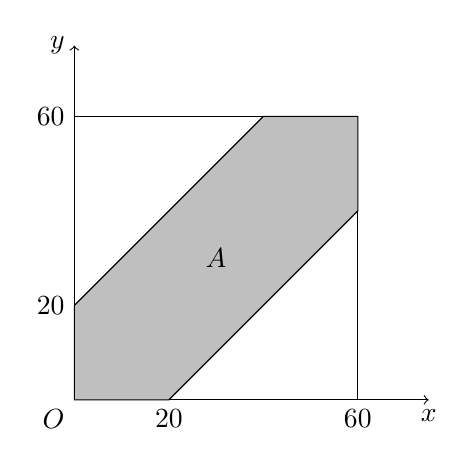
\begin{tikzpicture}[scale=0.6]
            % 坐标轴
            \draw[->] (0, 0)--(7.5, 0) node[below]{$x$};
            \draw[->] (0, 0)--(0, 7.5) node[left]{$y$};
            \node at (0, 0) [below left] {$O$};
            % 样本空间
            \draw (0,0) rectangle (6,6);
            \node at (6,0) [below] {60};
            \node at (0,6) [left] {60};
            \node at (1, 5) {$\varOmega$};
            % A
            \filldraw[fill=lightgray] (0,0) -- (0,2) -- (4,6) -- (6,6) -- (6,4) -- (2,0) -- cycle;
            \node at (3,3) {$A$};
            \node at (0,2) [left] {20};
            \node at (2,0) [below] {20};
        \end{tikzpicture}

        \caption{}
        \label{fig:会面问题}
    \end{figure}
\end{solution}

\question 甲乙两艘轮船驶向一个不能同时停泊两艘轮船的码头,它们在一昼夜  内到达的时间是等可能的.如果甲船的停泊时间是一小时,乙船的停泊时间是两小时,求它们中任何一艘都不需要等候码头空出的概率是多少?

\begin{solution}
    设甲、乙到达码头的时间分别为 $x,y$,则样本空间为
    $$
    \varOmega = \{ (x,y) \mid 0 \leqslant x \leqslant 24, 0 \leqslant y \leqslant 24 \}
    $$
    设事件 $A=$ ``甲乙都不需要等候码头空出'',该事件可以分为两种情况.如果甲先到达,则乙的到达时间应至少比甲晚一小时,即 $y \geqslant x+1$;如果乙先到达,则甲至少比乙晚到两小时,即 $x \geqslant y+2$.综合两种情况,事件 $A$ 可以表示为
    $$
    A = \{ (x,y) \mid y \geqslant x+1\ \text{或}\ y \leqslant x-2 \}
    $$
    如图 \ref{fig:几何概型-轮船停泊} 所示,所求概率为
    $$
    P(A) = \dfrac{\dfrac{23^2}{2} + \dfrac{22^2}{2}}{24^2} = \dfrac{1013}{1152}
    $$

    \begin{figure}[H]
        \centering
        \hspace{3em}
        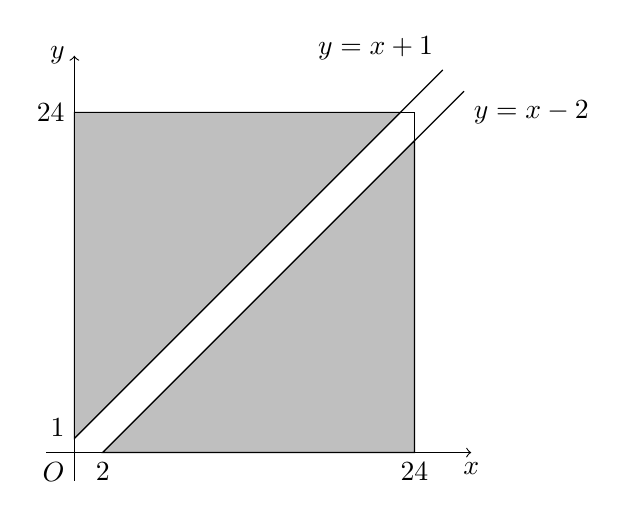
\begin{tikzpicture}[scale=0.18]
            % 坐标轴
            \draw[->] (-2, 0)--(28, 0) node[below]{$x$};
            \draw[->] (0, -2)--(0, 28) node[left]{$y$};
            \node at (0, 0) [below left] {$O$};
            % 定义特殊点
            \coordinate (O) at (0, 0);
            \coordinate (A) at (0, 24);
            \coordinate (B) at (24, 24);
            \coordinate (C) at (24, 0);
            \coordinate (D) at (0, 1);
            \coordinate (E) at (23, 24);
            \coordinate (F) at (2, 0);
            \coordinate (G) at (24, 22);
            % 曲线
            \draw (A) node[left]{$24$} -- (B) -- (C) node[below]{24};
            \draw (D) node[left, yshift=4pt]{1} -- (26, 27) node[above left]{$y=x+1$};
            \draw (F) node[below]{2} -- (27.5, 25.5) node[below right]{$y=x-2$};
            % 填充
            \filldraw[fill=lightgray] (D) -- (A) -- (E) -- cycle;
            \filldraw[fill=lightgray] (F) -- (G) -- (C) -- cycle;
        \end{tikzpicture}

        \caption{}
        \label{fig:几何概型-轮船停泊}
    \end{figure}
\end{solution}

\question 在长度为 $a$ 的线段内任取两点将其分为三段,求它们可以构成一个三角形的概率.

\begin{solution}
    设分成的三段长度分别为 $x, y$ 和 $a-x-y$,则有
    $$
    \begin{cases}
        0<x<a \\
        0<y<a \\
        0 < a-x-y < a
    \end{cases}
    $$
    其中 $0 < a-x-y < a$ 等价于 $0 < x+y < a$,则样本空间为
    $$
    \varOmega = \{ (x,y) \mid 0<x<a,\ 0<y<a,\ 0 < x+y < a \}
    $$

    设事件 $A = \text{``线段分成的三段可以构成三角形"}$.由于三角形中任意两边之和大于第三边,则事件 $A$ 发生的条件为
    $$
    \begin{cases}
        0 < x < y + (a-x-y) \\
        0 < y < x + (a-x-y) \\
        0 < a-x-y < x+y
    \end{cases}
    $$
    整理得
    $$
    A = \{ (x,y) \mid 0 < x < \dfrac{a}{2},\ 0 < y < \dfrac{a}{2},\ \dfrac{a}{2} < x+y < a \}
    $$
    如图 \ref{fig:example-三角形} 所示.则所求概率为
    $$
    P(A) = \dfrac{\dfrac{1}{2} \left( \dfrac{a}{2} \right)^2}{\dfrac{1}{2} a^2} = \dfrac{1}{4}
    $$

    \begin{figure}[H]
        \centering

        \begin{tikzpicture}[scale=1.1]
            % 坐标轴
            \draw[->] (-0.5, 0)--(3.5, 0) node[below]{$x$};
            \draw[->] (0, -0.5)--(0, 3.5) node[left]{$y$};
            \node at (0, 0) [below left] {$O$};
            % 定义特殊点
            \coordinate (A) at (0, 3);
            \coordinate (B) at (3, 0);
            \coordinate (C) at (0, 1.5);
            \coordinate (D) at (1.5, 0);
            \coordinate (E) at (1.5, 1.5);
            % 曲线
            \draw (A) node[left]{$a$} -- (B) node[below]{$a$};
            \draw (C) node[left]{$\dfrac{a}{2}$} -- (D) node[below]{$\dfrac{a}{2}$} -- (E) -- cycle;
            % 填充
            \filldraw[fill=lightgray] (C) -- (D) -- (E) -- cycle;
            % 区域标记
            \node at (1,1) {$A$};
            \node at (0.5, 2) {$\varOmega$};
        \end{tikzpicture}
        
        \caption{}
        \label{fig:example-三角形}
    \end{figure}
\end{solution}

\question 在平面上画有间隔为 $d$ 的等距平行线,向平面任意投掷一个边长为 $a, b, c$ (均小于 $d$)的三角形,求三角形与平行线相交的概率.

\begin{solution}
    三角形与平行线相交有三种情况:三角形的一个顶点在平行线上、一条边与平行线重合、两条边与平行线相交.由几何概型可知,前两种情况出现的概率为零,所以只需考虑两条边与平行线相交的概率.记 $P_{ab}, P_{bc}, P_{ac}$ 分别为两条边 $ab, bc, ac$ 与平行线相交的概率,则所求概率为
    $$
    p = P_{ab} + P_{bc} + P_{ac}
    $$
    设 $P_a, P_b, P_c$ 分别为边 $a,b,c$ 与平行线相交的概率,由蒲丰投针问题可得
    $$
    P_a = \dfrac{2a}{\pi d}, P_b = \dfrac{2b}{\pi d}, P_c = \dfrac{2c}{\pi d}
    $$
    $a$ 与平行线相交又能分成两种情况: $ab$ 与平行线相交、$ac$ 与平行线相交.因此
    $$
    P_a = P_{ab} + P_{ac}
    $$
    同理可得
    $$
    \begin{aligned}
        P_b = P_{ab} + P_{bc} \\
        P_c = P_{ac} + P_{bc}
    \end{aligned}
    $$
    因此,三角形与平行线相交的概率为
    $$
    p = P_{ab} + P_{bc} + P_{ac} = \dfrac{1}{2} (P_a + P_b + P_c) = \dfrac{a+b+c}{\pi d}
    $$
\end{solution}

\begin{note}
    \indent 本题是蒲丰投针问题的推广.该问题可以进一步推广到多边形及圆的情形.

    在平面上画有间隔为 $d$ 的等距平行线,向平面任意投掷一个周长为 $S_n$ 的凸多边形,且该凸多边形的直径小于 $d$ (凸多边形的直径是指多边形上任意两点之间的最大距离),则该凸多边形与平行线相交的概率为 $\dfrac{S_n}{\pi d}$.

    在平面上画有间隔为 $d$ 的等距平行线,向平面任意投掷一个半径为 $r \, (2r < d)$ 的圆,则该圆与平行线相交的概率为 $\dfrac{2r}{d}$.
\end{note}

\question 在半径为 $R$ 的圆内画平行弦,如果这些弦与垂直于弦的直径的交点 在该直径上的位置是等可能的,求任意画弦的长度大于 $R$ 的概率.

\begin{solution}
    设弦的中点与圆心的距离为 $x$,则样本空间为
    $$
    \varOmega = \{ x \mid 0 \leqslant x \leqslant R \}
    $$
    弦长为 $2 \sqrt{R^2 - x^2}$,当弦长大于 $R$ 时有 $2 \sqrt{R^2 - x^2} > R$,即 $x < \dfrac{\sqrt{3}}{2} R$.因此所求概率为
    $$
    p = \dfrac{\dfrac{\sqrt{3}}{2} R}{R} = \dfrac{\sqrt{3}}{2}
    $$

    \begin{figure}[H]
        \centering

        \begin{tikzpicture}
            \def\R{2}
            \def\x{2*\R/3}
            \pgfmathparse{sqrt(\R * \R - \x * \x)}

            \coordinate (O) at (0, 0); % 圆心
            \coordinate (M) at (0, \x); % 垂足
            \coordinate (A) at (\pgfmathresult, \x);
            \coordinate (B) at (-\pgfmathresult, \x);
            \coordinate (C) at (0, \R);

            \draw (O) circle (\R); % 圆
            \draw[fill] (O) circle (1.5pt); % 圆心
            \draw[dashed] (C) -- (0, -\R); % 直径
            \draw (A) -- (B); % 弦
            \draw[dashed] (B) -- (O); % 半径
            \node[right] at ($(O)!0.5!(M)$) {$x$};
            \node[below left] at ($(O)!0.5!(B)$) {$R$};
            
            % 直角符号
            \pic[draw=black, -, angle eccentricity=1.6, angle radius=0.2cm] {right angle = C--M--A};
        \end{tikzpicture}

        \caption{}
    \end{figure}
\end{solution}